\chapter{Preface} 

\section*{A free and open-source calculus \ \scalebox{0.5}{\includegraphics{figures/CClicense.eps}}} 

\vspace*{-0.15in}

Several fundamental ideas in calculus are more than 2000 years old.  As a formal subdiscipline of mathematics, calculus was first introduced and developed in the late 1600s, with key independent contributions from Sir Isaac Newton and Gottfried Wilhelm Leibniz.  Mathematicians agree that the subject has been understood rigorously since the work of Augustin Louis Cauchy and Karl Weierstrass in the mid 1800s when the field of modern analysis was developed, in part to make sense of the infinitely small quantities on which calculus rests.  Hence, as a body of knowledge calculus has been completely understood by experts for at least 150 years.  The discipline is one of our great human intellectual achievements:  among many spectacular ideas, calculus models how objects fall under the forces of gravity and wind resistance, explains how to compute areas and volumes of interesting shapes, enables us to work rigorously with infinitely small and infinitely large quantities, and connects the varying rates at which quantities change to the total change in the quantities themselves.

While each author of a calculus textbook certainly offers her own creative perspective on the subject, it is hardly the case that many of the ideas she presents are new.  Indeed, the mathematics community broadly agrees on what the main ideas of calculus are, as well as their justification and their importance; the core parts of nearly all calculus textbooks are very similar.  As such, it is our opinion that in the 21st century -- an age where the internet permits seamless and immediate transmission of information -- no one should be required to purchase a calculus text to read, to use for a class, or to find a coherent collection of problems to solve.  Calculus belongs to humankind, not any individual author or publishing company.  Thus, a main purpose of this work is to present a new calculus text that is \emph{free}.  In addition, instructors who are looking for a calculus text should have the opportunity to download the source files and make modifications that they see fit; thus this text is \emph{open-source}.  Since August 2013, \emph{Active Calculus} has been endorsed by the American Institute of Mathematics and its Open Textbook Initiative: \href{http://aimath.org/textbooks/}{\texttt{http://aimath.org/textbooks/}}.

Because the text is free, any professor or student may use the electronic version of the text for no charge.  A .pdf copy of the text may be obtained by download from
\begin{center} \href{http://gvsu.edu/s/xr}{\texttt{http://gvsu.edu/s/xr}}, \end{center}
where the user will also find a link to a print-on-demand for purchasing a bound, softcover version for about \$20.
Other ancillary materials, such as WeBWorK .def files, an activities-only workbook, and sample computer laboratory activities are available upon direct request to the author.  Furthermore, 
%A bound, printed copy of the text can be purchased for about \$** by visiting *****  
because the text is open-source, any instructor may acquire the full set of source files, again by request to the author at \href{mailto:boelkinm@gvsu.edu}{\texttt{boelkinm@gvsu.edu}}.  
This work is licensed under the Creative Commons Attribution-NonCommercial-ShareAlike 3.0 Unported License.  The graphic 
\begin{center}
\includegraphics{figures/CClicense.eps}
\end{center}
that appears throughout the text shows that the work is licensed with the Creative Commons, that the work may be used for free by any party so long as attribution is given to the author(s), that the work and its derivatives are used in the spirit of ``share and share alike,'' and that no party may sell this work or any of its derivatives for profit, with the following exception:  \emph{it is entirely acceptable for university bookstores to sell bound photocopied copies of the activities workbook to students at their standard markup above the copying expense.}  Full details may be found by visiting
\begin{center}
\href{http://creativecommons.org/licenses/by-nc-sa/3.0/}{\texttt{http://creativecommons.org/licenses/by-nc-sa/3.0/}}
\end{center} 
or sending a letter to Creative Commons, 444 Castro Street, Suite 900, Mountain View, California, 94041, USA. 

\section*{Active Calculus: our goals}

In \emph{Active Calculus}, we endeavor to actively engage students in learning the subject through an activity-driven approach in which the vast majority of the examples are completed by students.  Where many texts present a general theory of calculus followed by substantial collections of worked examples, we instead pose problems or situations, consider possibilities, and then ask students to investigate and explore.  Following key activities or examples, the presentation normally includes some overall perspective and a brief synopsis of general trends or properties, followed by formal statements of rules or theorems.  While we often offer plausibility arguments for such results, rarely do we include formal proofs.  It is not the intent of this text for the instructor or author to \emph{demonstrate} to students that the ideas of calculus are coherent and true, but rather for students to \emph{encounter} these ideas in a supportive, leading manner that enables them to begin to understand for themselves why calculus is both coherent and true.  This approach is consistent with the \href{http://launchings.blogspot.com/2011/07/the-worst-way-to-teach.html}{growing body of scholarship} that calls for students to be interactively engaged in class.

\newpage

Moreover, this approach is consistent with the following goals:

\begin{itemize}
   \item To have students engage in an active, inquiry-driven approach, where learners strive to construct solutions and approaches to ideas on their own, with appropriate support through questions posed, hints, and guidance from the instructor and text.
   \item To build in students intuition for why the main ideas in calculus are natural and true.  Often, we do this through consideration of the instantaneous position and velocity of a moving object, a scenario that is common and familiar.
   \item To challenge students to acquire deep, personal understanding of calculus through reading the text and completing preview activities on their own, through working on activities in small groups in class, and through doing substantial exercises outside of class time.  
   \item To strengthen students' written and oral communicating skills by having them write about and explain aloud the key ideas of calculus.
\end{itemize}

\section*{Features of the Text}

Instructors and students alike will find several consistent features in the presentation, including:

\begin{itemize}
	\item {\bf Motivating Questions.}  At the start of each section, we list 2-3 \emph{motivating questions} that provide motivation for why the following material is of interest to us.  One goal of each section is to answer each of the motivating questions.
	\item {\bf Preview Activities.} Each section of the text begins with a short introduction, followed by a \emph{preview activity}.  This brief reading and the preview activity are designed to foreshadow the upcoming ideas in the remainder of the section; both the reading and preview activity are intended to be accessible to students \emph{in advance} of class, and indeed to be completed by students before a day on which a particular section is to be considered.
	\item {\bf Activities.}  A typical section in the text has three \emph{activities}.  These are designed to engage students in an inquiry-based style that encourages them to construct solutions to key examples on their own, working individually or in small groups.  
	\item {\bf Exercises.}  There are dozens of calculus texts with (collectively) tens of thousands of exercises.  Rather than repeat standard and routine exercises in this text, we recommend the use of WeBWorK with its access to the National Problem Library and around 20,000 calculus problems.  In this text, there are approximately four challenging exercises per section.  Almost every such exercise has multiple parts, requires the student to connect several key ideas, and expects that the student will do at least a modest amount of writing to answer the questions and explain their findings.  For instructors interested in a more conventional source of exercises, consider the freely available text by Gilbert Strang of MIT, available in .pdf format from the MIT open courseware site via \href{http://gvsu.edu/s/bh}{\texttt{http://gvsu.edu/s/bh}}.
	\item {\bf Graphics.}  As much as possible, we strive to demonstrate key fundamental ideas visually, and to encourage students to do the same.  Throughout the text, we use full-color\footnote{To keep cost low, the graphics in the print-on-demand version are in black and white.  When the text itself refers to color in images, one needs to view the .pdf file electronically.} graphics to exemplify and magnify key ideas, and to use this graphical perspective alongside both numerical and algebraic representations of calculus.
	\item {\bf Links to Java Applets.}  Many of the ideas of calculus are best understood dynamically; java applets offer an often ideal format for investigations and demonstrations.  Relying primarily on the work of David Austin of Grand Valley State University and Marc Renault of Shippensburg University, each of whom has developed a large library of applets for calculus, we frequently point the reader (through active links in the .pdf version of the text) to applets that are relevant for key ideas under consideration.
	\item {\bf Summary of Key Ideas.}  Each section concludes with a summary of the key ideas encountered in the preceding section; this summary normally reflects responses to the motivating questions that began the section.
\end{itemize}


\section*{How to Use this Text}

This text may be used as a stand-alone textbook for a standard first semester college calculus course or as a supplement to a more traditional text.  Chapters \ref{C:1}-\ref{C:4} address the typical topics for differential calculus, while Chapters \ref{C:5}-\ref{C:8} provide the standard topics of integral calculus, including a chapter on differential equations (Chapter \ref{C:7}) and on infinite series (Chapter \ref{C:8}).

\subsection*{Electronically}

Because students and instructors alike have access to the book in .pdf format, there are several advantages to the text over a traditional print text.  One is that the text may be projected on a screen in the classroom (or even better, on a whiteboard) and the instructor may reference ideas in the text directly, add comments or notation or features to graphs, and indeed write right on the text itself.  Students can do likewise, choosing to print only whatever portions of the text are needed for them.  In addition, the electronic version of the text includes live html links to java applets, so student and instructor alike may follow those links to additional resources that lie outside the text itself.  Finally, students can have access to a copy of the text anywhere they have a computer, either by downloading the .pdf to their local machine or by the instructor posting the text on a course web site.

\subsection*{Activities Workbook}

Each section of the text has a preview activity and at least three in-class activities embedded in the discussion.  As it is the expectation that students will complete all of these activities, it is ideal for them to have room to work on them adjacent to the problem statements themselves.  As a separate document, we have compiled a workbook of activities that includes only the individual activity prompts, along with space provided for students to write their responses.  This workbook is the one printing expense that students will almost certainly have to undertake, and is available upon request.

There are also options in the source files for compiling the activities workbook with hints for each activity, or even full solutions.  These options can be engaged at the instructor's discretion, or upon request to the author.

%\subsection*{Print on Demand}

%\subsection*{Appendices}

\subsection*{Community of Users}

Because this text is free and open-source, we hope that as people use the text, they will contribute corrections, suggestions, and new material.  At this time, the best way to communicate such feedback is by email to Matt Boelkins at \href{mailto:boelkinm@gvsu.edu}{\texttt{boelkinm@gvsu.edu}}.  We have also started the blog \href{http://opencalculus.wordpress.com/}{\texttt{http://opencalculus.wordpress.com/}}, at which we will post feedback received by email as well as other points of discussion, to which readers may post additional comments and feedback.

\subsection*{Contributors}

The following people have generously contributed to the development or improvement of the text.  Contributing authors David Austin and Steven Schlicker have each written drafts of at least one chapter of the text.  The following contributing editors have offered significant feedback that includes information about typographical errors or suggestions to improve the exposition.

\begin{tabular}{l l l}
{\bf Contributing Editors:} & \ & \ \\
\ & David Austin & GVSU \\
\ & David Clark & GVSU \\
\ & Will Dickinson & GVSU \\
\ & Marcia Frobish & GVSU \\
\ & Mitch Keller & Washington \& Lee University \\
\ & Hugh McGuire & GVSU \\
\ & Ray Rosentrater & Westmont College \\
\end{tabular}
\newpage
\begin{tabular}{l l l}
{\bf Contributing Editors:} & \ & \ \\
\ & Luis Sanjuan & Conservatorio Profesional \\
\ & \ & \ \ de M\'{u}sica de \'{A}vila, Spain
\\
\ & Steven Schlicker & GVSU \\
\ & Brian Stanley & Foothill Community College \\
\ & Robert Talbert & GVSU \\
\ & Greg Thull & GVSU \\
%\ & Jerome Trouba & Ferris State University \\
\ & Sue Van Hattum & Contra Costa College \\
\end{tabular}


\section*{Acknowledgments}

This text began as my sabbatical project in the winter semester of 2012, during which I wrote the preponderance of the materials for the first four chapters.  For the sabbatical leave, I am indebted to Grand Valley State University for its support of the project and the time to write, as well as to my colleagues in the Department of Mathematics and the College of Liberal Arts and Sciences for their endorsement of the project as a valuable undertaking.

The beautiful full-color .eps graphics in the text are only possible because of David Austin of GVSU and Bill Casselman of the University of British Columbia.  Building on their collective longstanding efforts to develop tools for high quality mathematical graphics, David wrote a library of Python routines that build on Bill's PiScript program (available via \href{http://gvsu.edu/s/bi}{\texttt{http://gvsu.edu/s/bi}}), and David's routines are so easy to use that even I could generate graphics like the professionals that he and Bill are.  I am deeply grateful to them both.

For the print-on-demand version of the text (see \href{http://gvsu.edu/s/xr/}{\texttt{http://gvsu.edu/s/xr/}}), I am thankful for the support of Lon Mitchell and \href{http://orthogonalpublishing.com/}{Orthogonal Publishing L3C}.  Lon has provided considerable guidance on \LaTeX~and related typesetting issues, and has volunteered his time throughout the production process.  I met Lon at a special session devoted to open textbooks at the 2014 Joint Mathematics Meetings; I am grateful as well to the organizers of that session who are part of a growing community of mathematicians committed to free and open texts.  You can start to learn more about their work at \href{http://www.openmathbook.org/}{\texttt{http://www.openmathbook.org/}} and \href{http://aimath.org/textbooks/}{\texttt{http://aimath.org/textbooks/}}.

Over my more than 15 years at GVSU, many of my colleagues have shared with me ideas and resources for teaching calculus.  I am particularly indebted to David Austin, Will Dickinson, Paul Fishback, Jon Hodge, and Steve Schlicker for their contributions that improved my teaching of and thinking about calculus, including materials that I have modified and used over many different semesters with students.  Parts of these ideas can be found throughout this text.  In addition, Will Dickinson and Steve Schlicker provided me access to a large number of their electronic notes and activities from teaching of differential and integral calculus, and those ideas and materials have similarly impacted my work and writing in positive ways, with some of their problems and approaches finding parallel presentation here.  

Shelly Smith of GVSU and Matt Delong of Taylor University both provided extensive comments on the first few chapters of early drafts, feedback that was immensely helpful in improving the text.  As more and more people use the text, I am grateful to everyone who reads, edits, and uses this book, and hence contributes to its improvement through ongoing discussion. 

Finally, I am grateful for all that my students have taught me over the years.  Their responses and feedback have helped to shape me as a teacher, and I appreciate their willingness to wholeheartedly engage in the activities and approaches I've tried in class, to let me know how those affect their learning, and to help me learn and grow as an instructor.  Most recently, they've provided useful editorial feedback on an early version of this text. 

Any and all remaining errors or inconsistencies are mine.  I will gladly take reader and user feedback to correct them, along with other suggestions to improve the text. \\

\ \hfill Matt Boelkins, Allendale, MI
 
